\chapter{Identyfikacja modalna}

\section{Wiadomości wstępne}
Podstawowym celem pracy jest określenie zależności pomiędzy przyjętymi rozwiązaniami konstrukcyjnymi mostów kolejowych, a ich zachowaniem dynamicznym. Predykcja odpowiedzi, jak wspomniano wcześniej, możliwa jest dzięki rozwiązaniom numerycznym modeli MES poddanych odpowiednim obciążeniom. Na każdym etapie analiz trzeba zdawać sobie sprawę z niepewności, które mogą wystąpić przy konstruowaniu założeń. \cite{Brincker2015} zestawili różnego rodzaju parametry występujące w modelu i stopień niepewności, który im towarzyszy na etapie modelowania. Niepewności te przytoczono w tabeli \ref{table:uncertainitesModel}. Wyraźnie widać, że przyjęcie niektórych parametrów modelu w sposób bezkrytyczny może prowadzić do zupełnie nieodpowiednich rezultatów. Niektóre, związane np ze sztywnością szeroko rozumianych podpór czy połączeń śrubowych, mogą wypaczyć rezultaty i wprowadzić badacza w błąd na temat stanu i zachowania konstrukcji. Aby zbudować model, który będzie efektywnie odwzorowywał rzeczywiste zachowanie należy dołożyć wszelkich starań aby wyeliminować możliwe niepewności. Model taki może zostać poddany walidacji i kalibracji. Oba te pojęcia zostaną rozwinięte w następnych rozdziałach. Niemniej, aby model dostosować do rzeczywistych warunków należy mieć punkt odniesienia. W przypadku analizy statycznej takim odniesieniem mogą być pomiary statyczne ugięć, np. w trakcie próbnego obciążenia. W przypadku analizy dynamicznej, do porównania będą służyć charakterystyki modalne: częstotliwości i postaci drgań własnych oraz tłumienia. Parametry te można zaczerpnąć z literatury i doświadczenia na etapie projektowania. Na etapie badania rzeczywistej konstrukcji warto sięgnąć po narzędzie zwane identyfikacją modalną. Poniższy rozdział przytoczy podstawowe zagadanienia związane z analizą modalną, obliczeniami odpowiedzi dynamicznej i identyfikacją charakterystyk modalnych układu. Informacje te zostaną w dalszej części pracy zastosowane w obliczeniach numerycznych i optymalizacyjnych.



\begin{table} 
	\label{table:uncertainitesModel}
	\centering
	\caption{Niepewności najistotniejszych parametrów modeli numerycznych i modalnych na podstawie \cite{Brincker2015}}
	\rowcolors{1}{}{gray!10}
	\begin{tabular}{p{0.7\linewidth} | c}
		\toprule 
		Własność fizyczna   & Poziom niepewności \\
		\midrule
		Moduł sprężystości i gęstość masy dla stali i innych metali  &    1--5    \\
		Moduł sprężystości i gęstość masy dla betonu, drewna i zbrojonych włóknami materiałów & 5--20\\
		Warunki brzegowe z podłożem &    10-nieskończoność     \\
		Połączenia śrubowe & 10-nieskończoność\\
		Połączenia spawane & 2-10\\
		Masa całkowita & 1-5 \\
		Określana częstotliwość drgań własnych & 0.1-0.05\\
		Pomierzona odpowiedź & 0.2-2\\
		Określane postaci drgań własnych & 2-5\\ 
		Określane tłumienie & 5-20\\
		Współczynnik skalujący postaci drgań własnych & 5-30\\
		\bottomrule
	\end{tabular}
\end{table}



GDZIEŚ DO WSTĘPU: Drgania towarzyszą ludzkości od zawsze. Jakkolwiek trywialnie nie brzmiałoby to zdanie, wibracje występują w naszym otoczeniu przejawiając się często w sposób niepożądany: wywołują dyskomfort użytkowania, są odbierane jako hałas, powodują zjawiska zmęczeniowe czy w skrajnej sytuacji wywołują uszkodzenia i zniszczenia \parencite{Maia1997}. Wciąż postępujący rozwój nauki połączony z komputeryzacją i informatyzacją sprawiają, że używane materiały są coraz wytrzymalsze. Jednocześnie rośnie zapotrzebowanie na coraz większe, spektakularne konstrukcje. Te dwa czynniki połączone ze sobą sprawiają, że zachowanie dynamiczne struktury często decyduje o właściwościach użytkowych i wytrzymałościowych konstrukcji. 


W odpowiedzi na zapotrzebowanie, w sposób naturalny rozwinęła się dziedzina nauki zajmująca się opisem i modelowaniem zjawisk dynamicznych. Podstawowym narzędziem służącym identyfikacji parametrów modalnych i zachowania dynamicznego jest analiza modalna \teng{modal analysis}. Często Analiza modalna bywa określana jako identyfikacja modalna \teng{modal identification}. \parencite{Zhang2004} w pracy definiuje identyfikacje modalną jako gałąź szerszego pojęcia identyfikacji systemów, a jej celem jest budowa modelu matematycznego systemu dynamicznego poprzez pomiar i analizę zestawu danych wejściowych i wyjściowych. Z kolei \cite{Chmielewski1998} zwięźle precyzuje pojęcie modelu matematycznego dla zagadnień dynamiki budowli jako "równanie lub zbiór równań, które opisują ruch modelu obliczeniowego". \cite{Ewins2000} podaje trzy główne cele przeprowadzania analizy modalnej:
\begin{itemize}[noitemsep]
	\item ocena źródła drgań i ich przebiegu,
	\item weryfikacja modeli teoretycznych i przewidywanie zjawisk dynamicznych,
	\item identyfikacja charakterystyk materiałowych ciała poddanego wymuszeniu dynamicznemu (np. tłumienie, tarcie, wytrzymałość zmęczeniowa). 
\end{itemize}
Każdy z powyższych celów może być jedynie środkiem do osiągnięcia zupełnie innego celu. W rzeczywistości tak właśnie jest najczęściej o czym świadczy mnogość aplikacji analizy modalnej w bardzo różnych zagadnieniach dotyczących konstrukcji.

W poniższej pracy, tak jak w zdecydowanej większości innych opracowań, modele matematyczne będą oparte na trzech głównych zasadach \parencite{Maia1997}:
\begin{itemize}[noitemsep]
	\item system jest liniowy,
	\item obowiązuje zasada wzajemności Maxwell'a,
	\item system jest niezależny od czasu.
\end{itemize}


\section{Klasyfikacja metod analizy modalnej}

Identyfikacja modalna jest zbiorem technik, które są rozwijane dynamicznie od lat 60' XX w. Gwałtowny przyrost zainteresowania tym tematem wywołał głównie rozwój technik cyfrowych \parencite{Ewins2000}. Do tej pory powstało wiele różnych technik, których krótką klasyfikację z podziałem na główne kryteria podano w tym podrozdziale.

Matematyczne modele modalne mogą charakteryzować się różnym stopniem skomplikowania. Parametrami, które mogą opisywać model są postaci drgań własnych oraz powiązane z nimi częstotliwości i tłumienia modalne, a także masa i sztywność modalna. Z kolei metody analizy modalnej również różnią się pod względem informacji, którą mogą dostarczyć. Z tego względu wybór odpowiedniej metody powinien być świadomy i poparty przeglądem wielu technik, z których wybrana zostanie ta optymalna. Aspektami mogącymi wpłynąć na wybór metody są m.in.: czas potrzebny do implementacji (pierwszego użycia), informacje możliwe do uzyskania z modelu, możliwy wpływ założeń i uproszczeń, liczba parametrów potrzebnych do stworzenia modelu czy też stabilność rozwiązania. Przedstawiony podział opiera się na klasycznych kryteriach stosowanych przy klasyfikacji metod analizy modalnej. Istnieje wiele pozycji literaturowych, w których zainteresowany znajdzie dokładny opis wielu metod ze wskazówkami do ich użycia \parencite{Ewins2000,Maia1997,Zhang2004,Brincker2015,Rainieri2014}. 

Najogólniej analizę modalną można podzielić na dwie główne gałęzie zależne od typu stosowanej procedury, jej danych wejściowych i rezultatów: teoretyczną i eksperymentalną \parencite{Lengvarsky2013}. W niniejszej pracy wielokrotnie używane będą oba podejścia, dlatego autor zdecydował się na krótki ich opis. Ogólny schemat procedur teoretycznej i doświadczalnej analizy modalnej pokazano na rysunku \ref{fig:theExpProc}.  

\begin{figure}[h]
	\centering
	\subfloat[Procedura teoretyczna]{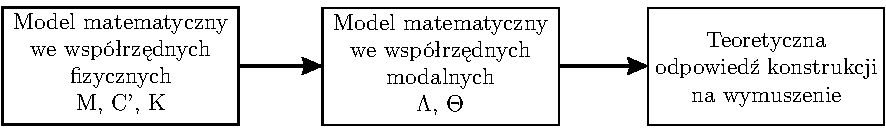
\includegraphics{/modal_analysis/schemat_theory_exper_a.pdf}
	\label{fig:theExpProcA}
	} \\
	\subfloat[Procedura doświadczalna]{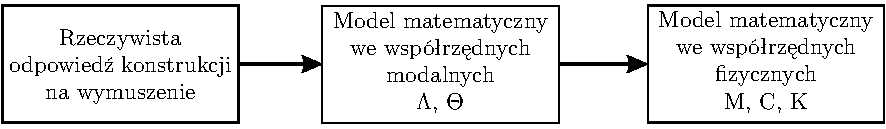
\includegraphics{/modal_analysis/schemat_theory_exper_b.pdf}
	\label{fig:theExpProcB}}
	\captionsetup{justification=centering}
	\caption{Porównanie procedur teoretycznej i doświadczalnej analizy modalnej}
	\label{fig:theExpProc}
\end{figure}

Metody teoretyczne opierają się na rozwiązaniach analitycznych lub numerycznych (rys. \ref{fig:theExpProcA}). Badanie zachowania dynamicznego rozpoczyna się od definicji struktury, najczęściej za pomocą modelu dyskretnego opisanego macierzami $\mathbf{M}, \mathbf{C}', \mathbf{K}$ oznaczającymi odpowiednio macierz mas, tłumienia i sztywności. Macierz tłumienia, w przypadku metod teoretycznych, jest to niewyznaczalna analitycznie macierz bazująca na doświadczeniach i rezultatach badań, stąd została oznaczona apostrofem $\mathbf{C'}$. Za pomocą przekształceń matematycznych (skrótowo opisanych w dalszej części tekstu) tworzony jest model matematyczny we współrzędnych modalnych. Uzyskiwane są charakterystyki modalne układu $\mathbf{\Lambda} \,\mathrm{i}\, \mathbf{\Psi}$ odpowiednio częstości drgań własnych, postaci drgań własnych i dodatkowo parametry opisujące przyjęty model tłumienia. Po uzyskaniu modelu matematycznego opisanego współrzędnymi modalnymi możliwe jest wyznaczenie odpowiedzi konstrukcji w czasie przy jej znanym wymuszeniu. Powyższy opis przedstawia pełną procedurę teoretyczną zakończoną wyznaczeniem odpowiedzi układu. Jednakże, jak wspomniano wcześniej, analiza modalna oraz jej metody są zróżnicowane z punktu widzenia skomplikowania. Zazwyczaj wybór metody zależy od zapotrzebowania na rezultaty. Zwłaszcza w przypadkach obliczeń inżynierskich często poprzestaje się na wyznaczeniu charakterystyk modalnych, które są następnie oceniane z punktu widzenia zagrożenia nadmiernymi efektami dynamicznymi.
Metody analityczne znajdują realne zastosowanie w przypadku obiektów, których opis ciągły nie jest złożony, a dyskretny ograniczony jedynie do niewielkiej liczby stopni swobody. Rzeczywiste konstrukcje są układami o nieskończonej liczbie stopni swobody. Niemniej, sprowadzenie ich do skończonej (choć zazwyczaj bardzo dużej) liczby stopni swobody pozwala otrzymać zadowalająco poprawne rezultaty. W przypadku dużej liczby stopni swobody najszerzej stosowane są metody przybliżone opierające się obliczeniach numerycznych, takie jak: metoda różnic skończonych (MRS) czy metoda elementów skończonych (MES). Teoretyczna analiza modalna ma wiele zalet. Pozwala uzyskać rezultaty relatywnie szybko i tanio. Wynika to z powszechności narzędzi do modelowania i obliczania konstrukcji. W obrębie modelowania realnych struktur współczesne oprogramowanie pozwala budować modele numeryczne praktycznie bez ograniczeń. Stosowane preprocesory graficzne pozwalają użytkownikowi na odwzorowanie nawet skomplikowanych kształtów geometrycznych. Rosnąca moc obliczeniowa komputerów przestaje być ograniczeniem, zwłaszcza przy obliczeniach statycznych modeli o znaczącej liczbie stopni swobody. Niepodważalną zaletą jest również dowolność sposobów obciążania i modyfikacji modelu numerycznego. Pomimo wielu niewątpliwych zalet, teoretyczna analiza modalna posiada ograniczenia, z których należy zdawać sobie sprawę. Przede wszystkim jakość rezultatów zależy wprost od jakości wprowadzonych przez użytkownika danych. (Potrzebne przykłady). W przypadku zagadnień dynamicznych kolejnym bardzo ważnym ograniczeniem jest brak analitycznej możliwości określenia tłumienia konstrukcji. Taką możliwość daje jedynie badanie doświadczalne na rzeczywistej konstrukcji. Metody analityczne i numeryczne są obszernie opisane w wielu publikacjach \parencite{Chmielewski1998,Chopra2012a,Rucka2014}. W dalszej części rozdziału zaprezentowano absolutne podstawy i założenia analitycznej analizy dynamicznej.


%\cite{Brincker2015} wskazuje na następujące źródła błędów i szacowane poziomy niepewności rezultatów analizy w zależności od rodzaju popełnionego błędów w definicji modelu MES (tab):

Doświadczalna analiza w odróżnieniu od wersji teoretycznej angażuje do identyfikacji warsztat badawczy. \cite{Ewins2000} definiuje ją jako zespół procesów związanych z badaniem elementów konstrukcji w celu uzyskania matematycznego opisu ich zachowania dynamicznego. Jest to definicja zbliżona do ogólniejszej podanej przez \cite{Zhang2004}, ale stawia szczególnie mocny akcent na aspekt badawczy. Jak przedstawiono na rysunku (rys. \ref{fig:theExpProcB}) ten typ analizy ma niejako odwrotny kierunek niż teoretyczna analiza modalna. W tym przypadku odpowiedź konstrukcji jest mierzona i na jej podstawie wyznaczane są wielkości opisujące model matematyczny: $\mathbf{\Lambda}$ i $\mathbf{\Psi}$. Następnie na dopiero ich podstawie możliwe jest przekształcenie na model matematyczny wyrażony we współrzędnych fizycznych: $\mathbf{M}, \mathbf{C}', \mathbf{K}$. 
Doświadczalna analiza modalna dzieli się na dwie główne odnogi związane z zakresem rejestrowanych danych w trakcie wykonywania eksperymentu. Pierwsza z nich to Eksperymentalna Analiza Modalna (EMA) \teng{Experimental Modal Analysis} wymaga pomiaru sił wymuszających oraz odpowiedzi konstrukcji na to wymuszenie. Druga to Operacyjna Analiza Modalna (OMA) \teng{Operational Modal Analysis}, która estymuje parametry modalne wyłącznie na podstawie pomierzonych efektów nieznanego wymuszenia. Wymuszenie to jednak nie może być dowolne, a ograniczenia przedstawione zostaną w dalszej części pracy. 

Kwestia pomiaru sił wymuszających wpływa na podstawowe różnice pomiędzy dwoma rodzinami metod: EMA i OMA. EMA najczęściej prowadzona jest w kontrolowanych warunkach i przez to pozwala dostarczyć bardziej szczegółowych i dokładniejszych informacji na temat zachowania dynamicznego konstrukcji. Jednakże w przypadku rzeczywistych konstrukcji inżynierskich (np. mosty) trudno jest stworzyć takie kontrolowane warunki. Obiekt musi zostać na czas pomiarów wyłączony z eksploatacji. Okazuje się to często niemożliwe z przyczyn proceduralnych, a na pewno kosztowne. Drugim zasadniczym ryzykiem jest potrzeba stworzenia takiego systemu wymuszenia, które wywoła mierzalną odpowiedź konstrukcji. W przypadku dużych konstrukcji inżynierskich może okazać się to trudne do zrealizowania ponieważ oddziaływania środowiskowe mogą wywoływać efekty oddziaływań porównywalne z kontrolowanym wymuszeniem. OMA praktycznie pozbywa się negatywnych skutków potrzeby kontroli wymuszenia. Badania prowadzone mogą być przy normalnej eksploatacji, a losowe oddziaływania środowiskowe zazwyczaj polepszają jakość wyników. Oczywiście odbywa się to kosztem dokładności rezultatów. Teoretyczne założenia metody są spełnione tylko w sposób przybliżony. Z tego względu serie pomiarowe zwykle muszą trwać znacznie dłużej, a interpretacja wyników wymaga większego doświadczenia.

\textbf{Połączenie obu typów analiz}

Obszerność zagadnień dotyczących analizy teoretycznej i identyfikacji modalnej wypełnia wiele tomów specjalistycznej literatury. Mimo chęci nie sposób przytoczyć je wszystkie z zadowalającą dokładnością. W rozdziale opisano najważniejsze według autora pojęcia których zrozumienie było kluczowe do  przeprowadzenia badań i analiz numerycznych.

\section{Teoretyczna analiza modalna}
\label{section: eigen}
Metody teoretycznej analizy modalnej są obszernie opisane w literaturze przedmiotu (cytowania). Ze względu na złożoność rzeczywistych konstrukcji, w praktyce mają one zastosowanie głównie w formie rozwiązań numerycznych.  Według przedstawionej na rysunku \ref{fig:theExpProcA} procedury metody teoretycznej analizy modalnej służą głównie dwóm celom: identyfikacji charakterystyk modalnych (częstotliwości i postaci drgań własnych) i wyznaczaniu odpowiedzi układu. Dla zrozumienia zagadnienia, metody analityczne najczęściej przedstawione są dla najprostszego przypadku układu z jednym stopniem swobody. Układ ten z reguły łatwo daje się uogólnić do układu o wielu stopniach swobody. Macierzowe równanie drgań wymuszonych dla tłumionego układu o skończonej liczbie stopni swobody przedstawiono we wzorze \ref{eq: mot_und}. 
\begin{equation} \label{eq: mot_und}
\vect{M} \vect{\ddot{x}}(t) +\vect{C} \vect{\dot{x}}(t)+ \vect{Kx}(t) = \vect{F}(t)
\end{equation}
gdzie $\vect{M},\vect{C},\vect{K}$ to odpowiednio macierze mass, tłumienia i sztywności, $\vect{x}$ to wektor współrzędnych uogólnionych (przemieszczeń lub obrotów punktu), $\vect{F}(t)$ to wektor uogólnionych sił wymuszających. Wzór \ref{eq: mot_dam} odpowiadający formule \ref{eq: mot_und} pozbawionej składnika reprezentującego opory ruchu opisuje ruch nietłumiony układu. 
\begin{equation} \label{eq: mot_dam}
\vect{M} \vect{\ddot{x}}(t) +\vect{Kx}(t) = \vect{F}(t)
\end{equation}

Drgania swobodne są procesem fizycznym spowodowanym zaburzeniem stanu równowagi, przez zaistnienie warunków początkowych. Macierzowe równanie ruchu drgań swobodnych, tłumionych opisane jest wzorem \ref{eq: mot_dam_free}, a nietłumionych wzorem \ref{eq: mot_und_free}. Od równań ruchu drgań wymuszonych, równania te różnią się brakiem składnika sił wymuszających.
\begin{equation} \label{eq: mot_dam_free}
\vect{M} \vect{\ddot{x}}(t) +\vect{C} \vect{\dot{x}}(t)+ \vect{Kx}(t) = \vect{0}
\end{equation}

\begin{equation} \label{eq: mot_und_free}
\vect{M} \vect{\ddot{x}}(t) +\vect{Kx}(t) = \vect{0}
\end{equation}


Okazuje się, że parametry modalne systemu są ściśle powiązane z rozwiązaniem algebraicznego problemu własnego równań drgań własnych. 

\subsection{Zagadnienie własne}
Identyfikacja modalna modelu matematycznego polegająca na wyznaczeniu częstotliwości i postaci drgań własnych najczęściej sprowadza się do rozwiązania zagadnienia własnego. Bardzo pozytywnym aspektem tej zależności jest to, że istnieje wiele prostych w aplikacji, wydajnych i dokładnych algorytmów pozwalających rozwiązać numerycznie zagadnienie własne \parencite{Golub2013}. Dzięki temu, właśnie ta metoda identyfikacji modalnej cieszy się największą popularnością wśród producentów oprogramowania do obliczania konstrukcji. Użytkownicy oprogramowania mogą bez większego wysiłku dokonać identyfikacji parametrów modalnych nawet złożonych modeli matematycznych. 
\subsubsection{Układ nietłumiony}
Z reguły przyjmuje się, że rozwiązanie zagadnienia własnego wykorzystuje równanie drgań swobodnych nietłumionych (\ref{eq: mot_und_free}). Należy zaznaczyć, że drgania własne nie opisują procesu fizycznego, a są jedynie matematyczną idealizacją drgań układu. W przypadku nietłumionym, dla każdego z modów, układ oscyluje wokół położenia równowagi z częstotliwością drgań własnych, a wszystkie stopnie swobody drgają w tej samej fazie. Oznacza to, że każdy z punktów osiąga swoje ekstremalne położenie w tej samej chwili. Podobnie wszystkie punkty znajdują się w położeniu równowagi w tym samym czasie. Poniżej przedstawiono rozwiązanie dla nietłumionego układu $N$ dynamicznych stopni swobody.

Założono rozwiązanie \ref{eq: mot_und_free} w postaci $\vect{x}(t)=\vect{\psi}e^{j\omega t}$ gdzie $\omega$ to częstość drgań własnych, $j=\sqrt{-1}$, a $\psi$ to niezerowy wektor postaci drgań własnych. Po podstawieniu rozwiązania i jego drugiej pochodnej ($\vect{\ddot{x}}(t)=-\vect{\psi} \omega^2 e^{j\omega t}$) do równia \ref{eq: mot_und_free} otrzymamy równanie \ref{eq: char_equation1}.

\begin{equation} \label{eq: char_equation1}
-\vect{M}\vect{\psi}\omega^2 e^{j\omega t} +\vect{K\psi}e^{j\omega t} = \vect{0}
\end{equation}
Dzieląc strony równania przez niezerową wartość $e^{j\omega t}$ otrzymujemy układ liniowych równań algebraicznych:
\begin{equation} \label{eq: char_equation2}
-\vect{M}\omega^2 \vect{\psi} +\vect{K\psi} = \vect{0}
\end{equation}
w którym dwie niewiadome do ustalenia to: $\psi$ - niezerowy wektor postaci drgań własnych oraz $\omega$ - częstość drgań własnych. Równanie to można zapisać w formie \ref{eq: char_equation3} z indeksami określającymi poszczególne mody drgań własnych. Liczba par odpowiadających sobie częstości $\omega_i$ i postaci drgań własnych $\psi_i$ jest równa liczbie $N$ stopni swobody. 
\begin{equation} \label{eq: char_equation3}
\omega^2_i \vect{M}\psi_i = \vect{K}\psi_i\qquad i=1,2,...,N
\end{equation}
Z kolei równanie \ref{eq: char_equation4} to reprezentacja uogólnionego problemu własnego, w którym $\lambda_i$ to wartość własna, a $u_i$ to wektor własny. Z porównania wzorów \ref{eq: char_equation3} i \ref{eq: char_equation4} wyraźnie widać powiązanie $\lambda_i=\omega^2_i$. Wynika z tego, że rozwiązanie numeryczne uogólnionego problemu własnego pozwala wprost uzyskać częstości $(\lambda_i=\omega^2_i)$ i postaci drgań własnych $(\psi_i)$. 
\begin{equation} \label{eq: char_equation4}
\lambda_i \vect{A}u_i = \vect{B}u_i
\end{equation}
Układ równań (\ref{eq: char_equation3}) ma nietrywialne rozwiązania tylko jeśli
\begin{equation} \label{eq: char_equation_det}
\det[\vect{K}-\omega^2_i \vect{M}] = \vect{0}
\end{equation}
Formuła \ref{eq: char_equation_det} jest znana jako równanie charakterystyczne zagadnienia własnego. Jeśli rozwinąć wyznacznik, otrzymamy wielomian stopnia $N$ względem $\omega^2_i$. Pierwiastkami równania \ref{eq: char_equation_det} są częstości drgań własnych $\omega_i$. Znając częstości własne $\omega_i$ z równania \ref{eq: char_equation3} można obliczyć odpowiadające wektory własne $\psi_i$ z dokładnością do stałego czynnika. Taki wynik bywa nieprzystępny w ocenie więc wektory poddawane mogą być normalizacji. Do najczęściej stosowanych metod normalizacji należy taka modyfikacja wektora tak aby maksymalna wartość bezwzględna spośród wszystkich elementu była równa jedności. Innym przykładem może być normalizacja wektorów tak aby wartość elementu dla danego stopnia swobody, we wszystkich wektorach była równa jedności.

Jeżeli macierze $\vect{M}$ i $\vect{K}$ ($\vect{A}$ i $\vect{B}$ wg \ref{eq: char_equation2}) są symetryczne i dodatnio określone o wartościach rzeczywistych to wartości oraz wektory własne są również rzeczywiste. W przypadku konstrukcji budowlanych macierz $\vect{K}$ jest zawsze dodatnio określona ponieważ warunki brzegowe zapewniają brak ruchu ciała jako bryły sztywnej. Nie jest to oczywiste dla innych niż budowlane struktur, takich jak np. samolot w locie \parencite{Chopra2012a}.


Postaci drgań własnych (wektory własne) odpowiadające różnym częstościom własnym spełniają warunki ortogonalności. W przypadku gdy $\omega_i \neq \omega_j$ prawdziwe są zależności \ref{eq: eigenvect_orto}. Ortogonalność wektorów własnych może być wykorzystana do weryfikacji obliczonych wektorów. 
\begin{equation} \label{eq: eigenvect_orto}
\vect{\psi}_i^{T}\vect{K\psi}_j = 0 \qquad \vect{\psi}_i^{T}\vect{M\psi}_j = 0
\end{equation}

Obliczone z równania \ref{eq: char_equation_det} wartości oraz wektory własne możemy przedstawić w postaci dwóch specjalnych macierzy. $N$ obliczonych wartości własnych zestawionych w macierz diagnonalną tworzy tak zwaną macierz widmową (\ref{eq: mat_spect}). Z kolei $N$ wektorów własnych zestawionych kolumnowo nazywamy macierzą modalną (\ref{eq: mat_modal}).

\begin{equation}  \label{eq: mat_spect}
\vect{\Omega}^2 =  
\begin{bmatrix} 
	\omega_{1}^2 & 0 			& \dots  & 0      \\ 
	0 		     & \omega_{2}^2 & \dots  & 0      \\
	\vdots       & \vdots       & \ddots & \vdots \\
	0 			 & 0 		    & \dots  & \omega_{N}^2 


\end{bmatrix}
\end{equation}

\begin{equation} \label{eq: mat_modal}
	\vect{\Psi} = [\psi_{i,j}]= 
	\begin{bmatrix} 
		\psi_{11} & \psi_{12} & \dots & \psi_{1N} \\ 
		\psi_{12} & \psi_{22} & \dots & \psi_{2N} \\
		\vdots    & \vdots    & \ddots & \vdots \\
		\psi_{N1} & \psi_{N2} & \dots & \psi_{NN} 
	
	
	\end{bmatrix}
	\qquad
	1\leq i,j \leq N.
\end{equation}

Dla układu o $N$ stopniach swobody możemy wyznaczyć $N$ par częstotliwości i postaci drgań własnych. Jednak w rzeczywistości rozwiązanie ogranicza się do wyznaczenia jedynie ograniczonej do kilkunastu (maksymalnie kilkuset) pierwszych par. Określenie "pierwszych" właściwe jest w przypadku kiedy wyznaczone częstości uporządkujemy w szeregu rosnącym
\begin{equation} \label{eq: eigenvalues_list}
0 \leq \omega_1  \leq \omega_2 \dots  \omega_{N-1} \leq  \omega_N
\end{equation}

W większości przypadków zagadnienie własne jest rozwiązywane numerycznie za pomocą maszyn cyfrowych. Metody numeryczne wykorzystują iteracyjne algorytmy do rozwiązania zagadnienia własnego. \cite{Chopra2012a} definiuje trzy główne kategorie algorytmów: 
\begin{itemize}[noitemsep]
	\item Metody iteracji wektora wykorzystujące właściwości równania (\ref{eq: char_equation3}),
	\item Metody transformacyjne korzystające z ortogonalności wektorów własnych,
	\item Metody iteracyjne wykorzystujące równanie charakterystyczne (\ref{eq: char_equation_det}).
\end{itemize}
Dla dużych systemów korzystne okazuje się łączenie algorytmów z tej samej bądź różnych kategorii co podnosi wydajność metody rozwiązania. W oprogramowaniu komercyjnym stosowane są złożone algorytmy takie jak metoda iteracji podprzestrzeni, metoda Lanczosa czy metoda gradientów Ritza. Wybór metody zależy również od wybranego solvera (silnika programu rozwiązującego równania). Algorytmy te różnią się pod względem wydajności, maksymalnej dokładności rozwiązania czy zbieżności. Ich wydajność może zależeć od liczby zadanych do wyznaczenia wartości własnych czy wielkości zadania. Więcej szczegółów odnośnie stosowanych metod rozwiązania zagadnienia własnego można odnaleźć w literaturze \parencite{Bathe2006,Wilson1983,Wilson1997,Fialko2000,Papadrakakis1993,Hughes1987,Chopra2012a}. W przypadku dobrej jakości oprogramowania komercyjnego informacje na temat używanych algorytmów powinny dostępne w pomocy do programu.

\subsubsection{Układ tłumiony}
Drgania swobodne tłumione układu określone są równaniem (\ref{eq: mot_dam_free}), które przytoczono ponownie poniżej:
\begin{equation} \label{eq: mot_dam_free2}
\vect{M} \vect{\ddot{x}}(t) +\vect{C} \vect{\dot{x}}(t)+ \vect{Kx}(t) = \vect{0}
\end{equation}
Rozwiązanie tego równania jest uzależnione od postaci tłumienia: klasycznego lub nieklasycznego. Tłumienie klasyczne zwane również proporcjonalnym \teng{classical damping, proportional damping} występuje w przypadku kiedy spełnione jest równanie (\ref{eq: class_damp}). 
\begin{equation} \label{eq: class_damp}
\vect{CM}^{-1}\vect{K} = \vect{KM}^{-1}\vect{C}
\end{equation}
Kiedy macierz $\vect{C}$ jest diagonalna to warunek (\ref{eq: class_damp}) jest spełniony. W takim przypadku wszystkie częstości drgań własnych są rzeczywiste i identyczne do tych wyznaczonych dla układu nietłumionego. W przypadku przeciwnym mamy do czynienia z tłumieniem nieklasycznym bądź nieproporcjonalnym \teng{nonclassical damping, nonproportional damping}. Dla tej sytuacji macierz $\vect{C}$ nie jest diagonalna, a wartości własne są zespolone. Szczegółowe informacje oraz metody rozwiązania przypadków dynamiki konstrukcji nieklasycznie tłumionych podano w \parencite{Caughey1961,Chopra2012a}. \cite{Inman1995} na przykładzie pokazali, że obliczanie struktur charakteryzujących się tłumieniem nieklasycznym za pomocą zagadnienia własnego bez uwzględnienia macierzy tłumienia możne prowadzić do błędnych rezultatów. Tak wyznaczone częstotliwości drgań będą różnić się od rzeczywistych, co może pociągnąć za sobą błędne wnioski odnośnie zakresu częstotliwości grożących rezonansem.
\subsection{Transformacja do współrzędnych normalnych} \label{section: transform_normal}
Rozważmy ponownie równanie ruchu układu MDOF (\ref{eq: mot_dam_free2}). Wiemy, że każdy wektor o długości $N$ może być przedstawiony jako kombinacja liniowa $N$ liniowo niezależnych wektorów. Przedstawmy zatem wektor przemieszczeń $\vect{x}$ jako kombinację wektorów własnych $\vect{\psi}$.
\begin{equation} \label{eq: normal_coord_komb}
	\vect{x} = \sum_{r=1}^{N} \vect{\psi}_r q_r=\vect{\Psi q}
\end{equation} 
gdzie współczynniki $q_r$ nazywane są współrzędnymi normalnymi \teng{modal coordinates, normal coordinates} i $\vect{q}=<q_1\,\,q_2\,\, \dots\,\, q_N>^T$. Załóżmy, że zagadnienie własne zostało rozstrzygnięte i wyznaczyliśmy macierz modalną $\vect{\Psi}$ (\ref{eq: mat_modal}). Aby uzyskać wartości współczynników $q_n$ dla danego $\vect{x}$, przemnóżmy obie strony równania \ref{eq: normal_coord_komb} przez $\vect{\psi}_n^T\vect{M}$:
\begin{equation} \label{eq: normal_coord_komb2}
	\vect{\psi}_n^T\vect{M}\vect{x} = \sum_{r=1}^{N} (\vect{\psi}_n^T\vect{M}\vect{\psi}_r) q_r
\end{equation} 

Ortogonalność wektorów własnych (\ref{eq: eigenvect_orto}) sprawia, że wszystkie składniki powyższej sumy są równe 0 poza tymi, w których $r=n$. Pomińmy więc znak sumy i zapiszmy 
\begin{equation} \label{eq: normal_coord_kom3}
	\vect{\psi}_n^T\vect{M}\vect{x} = (\vect{\psi}_n^T\vect{M}\vect{\psi}_n) q_n
\end{equation} 

\begin{equation} \label{eq: normal_coord_kom4}
	q_n = \frac{\vect{\psi}_n^T\vect{M}\vect{x}}{\vect{\psi}_n^T\vect{M}\vect{\psi}_n} 
\end{equation} 
Transformacja do współrzędnych normalnych jest istotnym elementem przewidywania odpowiedzi wymuszonych, liniowych układów MDOF z tłumieniem proporcjonalnym (p. \ref{section: mdof_response}).

%Należy wspomnieć, że uogólniony problem własny nie jest jedyną metodą rozwiązania macierzowego równania ruchu. Przy spełnieniu powyższych warunków możliwe jest również przekształcenie uogólnionego problemu własnego w odpowiedni standardowy (prosty) problem własny:
%\begin{equation} \label{eq: eige_stan_1}
%\vect{A}u_i = \lambda_i u_i
%\end{equation}
%Aby doprowadzić równanie \ref{eq: char_equation3} do postaci standardowego problemu własnego wymagane jest wyznaczenie macierzy odwrotnej $\vect{M}^{-1}$. W przypadku kiedy jest to możliwe (na przykład przy pomocy dekompozycji Choleskiego) należy pomnożyć lewostronnie strony równania przez $\vect{M}^{-1}$ co pozwala uzyskać postać (\ref{eq: eige_stan_2}). Ponownie widoczne jest podobieństwo pomiędzy równaniami i powiązanie $(\lambda_i=\omega^2_i)$. Sprowadzenie do standardowego problemu własnego bywa korzystne z punktu widzenia rozwiązania numerycznego. 
%\begin{equation} \label{eq: eige_stan_2}
%\vect{M}^{-1}\vect{K}\psi_i=\omega^2_i\psi_i
%\end{equation}

\subsection{Odpowiedź systemów dynamicznych o jednym stopniu swobody} \label{section: sdof_response}

Przegląd metod pozwalających wyznaczyć odpowiedź konstrukcji poddanej wymuszeniu wypada zacząć klasycznie od układu z jednym stopniem swobody. W przypadku liniowego układu SDOF obciążonego siłą zewnętrzną, równanie ruchu jest liniowym równaniem różniczkowym drugiego rzędu (\ref{eq: eq_mot_sdof}). Znając warunki początkowe $x(0)$ i $\dot{x}(0)$ możemy traktować zadanie jako w pełni sformułowane. Dla konstrukcji wstępnie nieobciążonej dynamicznie przemieszczenie i prędkość początkowe można przyjąć jako równe zeru.
\begin{equation} \label{eq: eq_mot_sdof}
	m\ddot{x}+c\dot{x}+k{x}=f(t)
\end{equation}
Dla tak sformułowanego problemu istnieją cztery podstawowe metody wyznaczenia odpowiedzi dynamicznej:
\begin{itemize}[noitemsep]
	\item klasyczne rozwiązanie równań różniczkowych,
	\item wykorzystanie całki Duhamela,
	\item rozwiązanie w dziedzinie częstotliwości,
	\item wykorzystanie metod numerycznych.
\end{itemize}
Dla porządku powyższe metody zostaną w dalszej części krótko opisane. Dokładny opis metod jest przedstawiony w wielu podstawowych pozycjach literaturowych dotyczących dynamiki budowli \parencite{Clough1975,Chmielewski1998,Chopra2012a}.

\subsubsection{Metoda klasyczna}

Rozwiązanie liniowego równania różniczkowego o stałych współczynnikach jakim jest równanie ruchu składa się z rozwiązania całki ogólnej i szczególnej, a następnie zsumowaniu ich. Równanie ruchu jest rzędu drugiego stąd do wyznaczenia pozostają dwie zmienne całkowania. Z kolei do ich wyznaczenia wykorzystane są warunki początkowe. $\bm{OGRANICZENIA}$

\subsubsection{Całka Duhamela}

Metoda rozwiązania równania ruchu układu SDOF za pomocą całki Duhamela polega na przekształceniu funkcji obciążenia $f(t)$ na sekwencję nieskończenie krótkich impulsów. Przykładając impulsowe, jednostkowe wymuszenie (delta Diraca) do układu (\ref{eq: eq_mot_sdof}), dla odpowiednich warunków początkowych otrzymuje się rozwiązanie w postaci odpowiedzi impulsowej, inaczej zwanej impulsową funkcją przejścia \teng{unit response function}. Aby uzyskać odpowiedź układu w czasie $t$ sumuje się wszystkie odpowiedzi impulsowe do chwili czasowej $t$. W przypadku całkowalnej funkcji wymuszenia, całka Duhamela może być alternatywą do rozwiązania metodą klasyczną. Dla eksperymentalnych funkcji wymuszenia, całkę Duhamela można wyznaczyć metodami numerycznymi. W tym przypadku odpowiedź będzie wyznaczona w dyskretnych chwilach czasowych. Należy jednak wspomnieć, w przypadku angażowania metod numerycznych całka Duhamela nie jest najwydajniejszym rozwiązaniem. Dodatkowo, ze względu na wykorzystywaną superpozycję, rozwiązanie to jest ograniczone wyłącznie do układów liniowych.

\subsubsection{Metoda przejścia do dziedziny częstotliwości}

Metoda przejścia do dziedziny częstotliwości \teng{frequency-domain method} wykorzystuje właściwości przekształceń Laplace'a lub Fourier'a. Dla układu SDOF (\ref{eq: eq_mot_sdof}) wykonuje się wybrane przekształcenie funkcji wymuszenia $f(t)$ uzyskując $F(\omega)$. $F(\omega)$ można określić jako amplitudy wszystkich składników harmonicznych, które składają się na wymuszenie $f(t)$ Przekształcenie $X(\omega)$ rozwiązania równania różniczkowego $x(t)$ można z kolei opisać następująco
\begin{equation}
	X(\omega)=H(\omega)F(\omega)
\end{equation}
gdzie $H(\omega)$ to odpowiedź zespolona w dziedzinie częstotliwości nazywana też funkcją przenoszenia lub transmitancją \teng{complex frequency-response function (FRF)}. Funkcja przenoszenia $H(\omega)$ opisuje odpowiedź układu w dziedzinie częstotliwości przy wymuszeniu harmonicznym. Ostatnim krokiem metody jest wyznaczenie rozwiązania $x(t)$ poddając $X(\omega)$ odwrotnemu przekształceniu (Fourier'a bądź Laplace'a). Tak uzyskany rezultat $x(t)$ można traktować jako określenie odpowiedzi harmonicznych układu na każdy z składników wymuszenia. Te cząstkoweg odpowiedzi te są następnie sumowane w celu uzyskania całkowitej odpowiedzi $x(t)$. Ponownie, metoda ta bezpośrednio może być stosowana tylko dla prostych funkcji wymuszenia $f(t)$. Jeżeli funkcja wymuszenia jest określona numerycznie, odpowiednie przekształcenia można przeprowadzić np. z użyciem algorytmu dyskretnej transformaty Fouriera w wariancie szybkiej transformaty Fourier'a \teng{Fast Fourier Transform (FFT)}.

\subsubsection{Metody numeryczne}

Zastosowanie powyższych trzech metody wyznaczania odpowiedzi dynamicznej ograniczone jest tylko do układów liniowych. Wspomniano również, że stają się niepraktyczne lub wręcz niemożliwe do zastosowania w przypadku skomplikowanych, zmiennych w czasie funkcji wymuszenia $f(t)$. W takich niekorzystnych okolicznościach z pomocą przychodzą metody numeryczne. Co więcej, okazuje się, że w przypadkach liniowych układów metody te są również konkurencyjne dla metod analitycznych. 

Stworzono wiele metod i algorytmów numerycznych służących skutecznemu rozwiązaniu równań ruchu. Powstało również wiele pozycji traktujących o tym zagadnieniu (LITERATRA). Z tego względu przytoczono tylko podstawowe pojęcia i założenia dotyczące istoty rozwiązań numerycznych.

Metody numeryczne w głównej mierze opierają się na mechanizmie kroku czasowego \teng{time-step} (p. \ref{section: mdof_response}). Zwykle nie jest to rozwiązanie ścisłe. Metody dostarczają jedynie przybliżonych rozwiązań, dlatego też muszą spełniać następujące kryteria:
\begin{itemize}[noitemsep]
	\item zbieżności \teng{convergence} - wraz ze zmniejszeniem kroku czasowego, rozwiązanie powinno zmierzać do rozwiązania dokładnego,
	\item stabilności \teng{stability} - rozwiązanie powinno być stabilne pomimo występowania błędów zaokrągleń,
	\item dokładności \teng{accuracy} - rozwiązanie powinno być dostatecznie bliskie rozwiązanie dokładnego.
\end{itemize}
Wśród metod numerycznych, które okazały się skuteczne w rozwiązaniach problemów możemy wyróżnić trzy główne:
\begin{itemize}[noitemsep]
\item metoda interpolacji funkcji wymuszającej,
\item metoda różnic skończonych,
\item metoda średniego lub liniowego przyspieszenia w przedziale różnicowym, oparte na metodzie Newmark'a.
\end{itemize}
Pomimo, że powyższe metody są opisane dla układu SDOF, są łatwo uogólniane i praktycznie wykorzystywane do obliczania układów MDOF. Algorytm metody Newmark'a jest najpowszechniej używany w obliczeniach konstrukcji inżynierskich oraz został wykorzystany w niniejszej pracy. Stąd w następnym podrozdziale zawarto zwięzły opis jego działania.


\subsection{Odpowiedź systemów dynamicznych o skończonej liczbie stopni swobody (MDOF)} \label{section: mdof_response}

Systemy o skończonej liczbie stopni swobody mogą charakteryzować się tłumieniem klasycznym (proporcjonalnym) bądź nieklasycznym (nieproporcjonalnym). Mogą być liniowe lub nieliniowe geometrycznie lub materiałowo. Czynniki te mają wpływ na wybór metody przewidywania odpowiedzi takiego układu. Macierzowe równanie ruchu dla układu o $N$ stopniach swobody możemy zapisać jako $N$ równań różniczkowych w formie (\ref{eq: mot_und}) dla wygody ponownie opisanej równaniem (\ref{eq: mot_und_num})
\begin{equation} \label{eq: mot_und_num}
	\vect{M} \vect{\ddot{x}}(t) +\vect{C} \vect{\dot{x}}(t)+ \vect{Kx}(t) = \vect{F}(t)
\end{equation}
 Modelem z tłumieniem proporcjonalnym, z wystarczającym przybliżeniem, można opisać większość badanych struktur. Odpowiedź układów ograniczonych do kilku stopni swobody może być wyznaczana przez rozwiązanie równania różniczkowego \ref{eq: mot_und_num}. W przypadku większej liczby stopni swobody zwykle wykorzystuje się metody numeryczne. Jak wiemy z rozdziału \ref{section: eigen}, dla takich układów zawsze możliwe jest wyznaczenie częstotliwości i postaci drgań własnych. Co więcej, opisujące je macierzowe równanie ruchu można przekształcić za pomocą metody transformacji własnej do postaci zależnej od współrzędnych modalnych. W takiej formie równanie to jest zbiorem równań rozwikłanych. Z tego względu można wyznaczyć odpowiedź dla każdego modu (zestawu jednej częstotliwości i postaci własnej oraz towarzyszącego tłumienia) osobno, a następnie złożyć je w celu wyznaczenia odpowiedzi całkowitej. Dodatkowo, każda odpowiedź modalna może być wyznaczona jako funkcja czasu przez analizę układu SDOF. Równania SDF mogą być oczywiście rozwiązane wszystkimi przytoczonymi wcześniej wymienionymi metodami - w tym numerycznymi.
 
 W przypadku kiedy mamy do czynienia z układem o tłumieniu nieproporcjonalnym, klasyczne parametry modalne nie mogą być wyznaczone, a równania ruchu nie mogą być rozwikłane. Takie systemy można analizować dwiema metodami: poprzez przekształcenie równań ruchu na wektory własne obliczone w zespolonym zagadnieniu własnym lub poprzez bezpośrednie całkowanie nierozwikłanych równań różniczkowych. Druga metoda wykorzystuje metody numeryczne co wynika z braku zamkniętych rozwiązań analitycznych nawet dla analitycznie opisanych funkcji obciążenia. Metody numeryczne muszą być stosowane również w przypadku kiedy układ jest nieliniowy (niezależnie czy materiałowo, czy geometrycznie). W przypadku braku założenia o liniowości wybór metody nie jest uzależniony od tego, czy tłumienie jest proporcjonalne, czy też nie jest.
 
 Zachowując porządek i kompletność wywodu poniżej przedstawiono krótki zarys dwóch podstawowych metod wyznaczania odpowiedzi układów dyskretnych o skończonej liczbie stopni swobody.
 
 \subsubsection{Metoda superpozycji modalnej}
Rozpatrzmy układ MDOF, liniowy o tłumieniu proporcjonalnym dany równaniem \ref{eq: mot_und_num}. Wiemy, że wektor przemieszczeń $\vect{x}$ może być zapisany za pomocą współrzędnych normalnych (p. \ref{section: transform_normal}) co powtórzono dla wygody poniżej:

\begin{equation} \label{eq: superposition_modal_1_przytocz}
	\vect{x}(t) = \sum_{r=1}^{N} \vect{\psi}_r q_r(t)=\vect{\Psi q}(t)
\end{equation} 

Podstawmy \ref{eq: superposition_modal_1} do równania \ref{eq: mot_und_num}
\begin{equation} \label{eq: superposition_modal_2_podstaw}
	\sum_{r=1}^{N} \vect{M} \vect{\psi}_r \ddot{q}_r(t) +\sum_{r=1}^{N} \vect{C}\vect{\psi}_r \dot{q}_r(t) + \sum_{r=1}^{N} \vect{K}\vect{\psi}_r q_r(t) = \vect{F}(t)
\end{equation} 
Następnie przemnóżmy z lewej strony każdy składnik przez $\vect{\psi}_n^T$ otrzymując:
\begin{equation} \label{eq: superposition_modal_3_przemnoz}
	\sum_{r=1}^{N} \vect{\psi}_n^T \vect{M} \vect{\psi}_r \ddot{q}_r(t) +\sum_{r=1}^{N} \vect{\psi}_n^T \vect{C}\vect{\psi}_r \dot{q}_r(t) + \sum_{r=1}^{N} \vect{\psi}_n^T \vect{K}\vect{\psi}_r q_r(t) = \vect{\psi}_n^T \vect{F}(t)
\end{equation} 
Podobnie jak w punkcie \ref{section: transform_normal}, ortogonalność wektorów własnych $\vect{\psi}$ sprawia, że wszystkie składniki sum, w których $r\neq n$, zerują się. Możemy więc zapisać zredukowane równanie w postaci
\begin{equation} \label{eq: superposition_modal_4_orto}
	 (\vect{\psi}_n^T \vect{M} \vect{\psi}_n )\ddot{q}_n(t) + (\vect{\psi}_n^T \vect{C}\vect{\psi}_n) \dot{q}_n(t) + (\vect{\psi}_n^T \vect{K}\vect{\psi}_n) q_n(t) = \vect{\psi}_n^T \vect{F}(t)
\end{equation} 
Zauważmy, że iloczyny zawarte w nawiasach są skalarami. Uprośćmy więc zapis do następującej formy:
\begin{equation} \label{eq: superposition_modal_5_uprosc}
	\mathcal{M}_n\ddot{q}_n(t) + \mathcal{C}_n\dot{q}_n(t) + \mathcal{K}_n q_n(t) = \mathcal{F}_n(t)
\end{equation} 
gdzie:
\begin{equation} \label{eq: superposition_modal_6_podstawki}
	\mathcal{M}_n= \vect{\psi}_n^T \vect{M} \vect{\psi}_n \qquad 
	\mathcal{C}_n= \vect{\psi}_n^T \vect{C} \vect{\psi}_n \qquad 
	\mathcal{K}_n= \vect{\psi}_n^T \vect{K} \vect{\psi}_n \qquad
	\mathcal{F}_n(t)= \vect{\psi}_n^T \vect{F}(t)
\end{equation} 
Okazuje się, że wszystkie powyższe przekształcenia doprowadzają do tego, że (\ref{eq: superposition_modal_5_uprosc}) jest równaniem o jednym stopniu swobody dla $n$-tej współrzędnej normalnej odpowiadającej $n$-tej postaci drgań. Z tego względu współczynniki $\mathcal{M}_n,\:\mathcal{C}_n,\:\mathcal{K}_n,\:\mathcal{F}_n(t)$ nazywane są odpowiednio uogólnioną masą, uogólnionym tłumieniem, uogólnioną sztywnością i uogólnioną siłą dla $n$-tej postaci własnej \teng{generalized mass, generalized damping, generalized stiffness, generalized force}. Równanie to możemy rozwiązać wszystkimi metodami dotyczącymi układów SDOF przedstawionymi w (p. \ref{section: sdof_response}). Warto też zwrócić uwagę, że wartości $\mathcal{M}_n,\:\mathcal{C}_n,\:\mathcal{K}_n,\:\mathcal{F}_n(t)$ są uzależnione jedynie od pojedynczej postaci drgań $\vect{\psi}_n$. Naturalnie więc, jeśli znamy tylko jeden mod $\vect{\psi}_n$, możemy wyznaczyć odpowiadający mu parametr $q_n$ bez znajomości pozostałych modów.
Jeśli współczynniki normalne $q_n$ zostały wyznaczone dla $N'$ wybranych (najczęściej kilku istotnych) modów, to wkład $n$-tego modu w całkowitą wartość przemieszczeń $\vect{x}(t)$ wyznaczyć można następująco
\begin{equation} \label{eq: modal_sup_contr}
	\vect{x}_n(t) = \vect{\psi}_n q_n(t)
\end{equation}
a wykorzystując równania (\ref{eq: superposition_modal_1_przytocz}) i (\ref{eq: modal_sup_contr}) obliczyć przemieszczenie całkowite
\begin{equation}
		\vect{x}(t) = \sum_{r=1}^{N'} \vect{x}_n(t)
\end{equation}

Sumowanie wkładu poszczególnych postaci drgań w przemieszczenie całkowite jest par excellence superpozycją. Stąd też nazwa: "metoda superpozycji modalnej". Należy wspomnieć o paru istotnych założeniach mogących wpłynąć na zastosowanie tej metody. Jak już wcześniej wspomniano, może być ona wykorzystana tylko w układach liniowych (ze względu na superpozycję) i tłumionych proporcjonalnie. W przypadku tłumienia nieproporcjalnego przekształcenie równania (\ref{eq: superposition_modal_3_przemnoz}) do (\ref{eq: superposition_modal_4_orto}) nie będzie prawdziwe. Warto również pamiętać, że wynikowe przemieszczenia $\vect{x}(t)$ są niezależne od normalizacji wektorów własnych, natomiast współrzędne normalne $q_n(t)$ są od niej ściśle zależne. 

\subsubsection{Metoda całkowania bezpośredniego równań ruchu - Newmarka}
Metoda Newmarka jest algorytmem opartym na koncepcji kroku czasowego i metodach numerycznych. Zgodnie z koncepcją kroku czasowego całkowity czas podzielony jest na serię kroków czasowych, zwykle o stałej wartości $\Delta t$. Polega on na dyskretyzacji siły wymuszającej i odpowiedzi układu poprzez określenie ich wyłącznie w wybranych chwilach czasowych. Rozpatrzmy ponownie równanie ruchu MDOF:
\begin{equation}
	\vect{M}\vect{\ddot{x}}+\vect{C}\vect{\dot{x}}+\vect{K}\vect{x} = \vect{F}(t)
\end{equation} 
Dokonajmy dyskretyzacji i przedstawmy siłę wymuszającą $F(t)$ określoną dla $t\in<0,t_k>$ jako zestaw dyskretnych wartości w chwilach czasowych $t_i$:
\begin{equation}
	\vect{F}_i=\vect{F}(t_i) \qquad i = 0,1,2\dots N-1,N
\end{equation}
gdzie $t_N\leq t_k$. Krokiem czasowym nazywamy różnice pomiędzy kolejnymi zdyskretyzowanymi chwilami czasowymi:
\begin{equation}
	\Delta t_i = t_{i+1}-t_i
\end{equation}
Jest on zazwyczaj przyjmowany jako stały, ale nie jest to konieczne. Tak jak wymuszenie, odpowiedź również podlega dyskretyzacji w chwilach $t_i$, a więc równanie ruchu można zapisać w nowej formie
\begin{equation} \label{eq: motion_time_step}
	\vect{M}\vect{\ddot{x}}_i+\vect{C}\vect{\dot{x}}_i+\vect{K}\vect{x}_i = \vect{F}_i
\end{equation}
Znając warunki początkowe $\vect{x}(0)$ i $\vect{\dot{x}}(0)$ algorytmy wykorzystywane w metodach numerycznych potrafią wyznaczyć rozwiązania równania w kolejnych krokach $i = 1,2\dots N-1,N$. 

Rodzina metod numerycznych opartych na koncepcji kroku czasowego została rozwinięta przez Nathana M. Newmarka \parencite{Newmark1959}. Wykorzystuje ona dwa podstawowe równania:
\begin{subequations} \label{eq: newmark}
	\begin{align}
		\vect{\dot{x}}_{i+1} &= \vect{\dot{x}}_{i} + [(1-\gamma)\Delta t)]\vect{\ddot{x}}_{i} + (\gamma\Delta t)\vect{\ddot{x}}_{i+1} 
		\label{eq: newmark_a}\\
		\vect{x}_{i+1} &= \vect{x}_{i} + (\Delta t)\vect{\dot{x}}_{i} + [(0.5-\beta)(\Delta t)^2)]\vect{\ddot{x}}_{i}+ (\beta(\Delta t)^2)\vect{\ddot{x}}_{i+1} 
		\label{eq: newmark_b}
	\end{align}
\end{subequations}
gdzie współczynniki $\beta$ i $\gamma$ definiują zmienność przyspieszeń w trakcie kroku czasowego i istotnie wpływają na stabilność i dokładność metody. Ze względu na oba te warunki, przy braku modyfikacji algorytmu, parametry powinny mieć następujące wartości: $\gamma = \frac{1}{2}$, a $ \frac{1}{6}\leq \beta \leq \frac{1}{4}$. Na skrajach zalecanego przedziału wartości parametru $\beta$ występują dwa przypadki szczególne, w których przyspieszenie ma określony charakter w kroku czasowym:
\begin{itemize}[noitemsep]
	\item przyspieszenie stałe - $\gamma = \frac{1}{2},\: \beta = \frac{1}{4}$
	\item przyspieszenie zmienne liniowo - $\gamma = \frac{1}{2},\: \beta = \frac{1}{6}$
\end{itemize}[noitemsep]
Metoda numeryczna do wyznaczenia trzech niewiadomych $\vect{\ddot{x}}_{i+1}$, $\vect{\dot{x}}_{i+1}$ i $\vect{x}_{i+1}$ wymaga układu trzech równań macierzowych. Zatem dwa zaproponowane równania \ref{eq: newmark_a} i \ref{eq: newmark_b}, połączone z równaniem równowagi (\ref{eq: motion_time_step}) zapewnionym na końcu kroku czasowego, pozwalają wyznaczyć przemieszczenia, prędkość i przyspieszenia w chwili $t_{i+1}$. Ze względu na występowanie w równaniach (\ref{eq: newmark}) składników w chwili czasowej $i+1$ po obu stronach równania, algorytm musi mieć charakter iteracyjny. Jednakże istnieją modyfikacje równań, które dla układów liniowych pozwalają rozwiązać układ w jednym kroku.


\section{Operacyjna analiza modalna (OMA)}
\subsection{Koncepcja OMA}
W ogólności doświadczalna analiza modalna to proces korelacji charakterystyk dynamicznych modelu matematycznego, z fizycznymi właściwościami systemu opisanego rezultatami pomiarów. Przypomnijmy, że w OMA do procesu estymacji parametrów modalnych używane są tylko pomiary odpowiedzi konstrukcji. Różni ją to od EMA, w której mierzone są zarówno wymuszenia jak i odpowiedź. 
Fundamentem wszystkich metod OMA jest założenie, że badana struktura obciążona jest wymuszeniem o widmie zbliżonym do białego szumu. Oznacza to, żę energia konstrukcji jest rozłożona w szerokim paśmie częstotliwości, które zawiera wszystkie interesuje badacza mody do identyfikacji. Z oczywistych względów idealne wymuszenie o charakterystyce białego szumu nie jest możliwe. Większość metod radzi sobie z tym brakiem, jednak najważniejsze jest, żeby wszystkie interesujące mody były odpowiednio wzbudzone, tak aby ich wkład był wychwycony przez przyrządy pomiarowe. \cite{Brincker2015} tłumaczą tę koncepcję za pomocą fikcyjnego, kolorowego filtru obciążenia. Zaproponowano, że kolorowe obciążenie może być traktowanego jako wynik obciążenia kolorowego filtru (zgodnego z obciążeniem) przez idealnie biały szum. Udowodniono, że takie podejście nie zmienia fizycznych modów systemu. Należy jednak pamiętać, że metody OMA w tym przypadku dokonają identyfikacji modalnej zarówno struktury fizycznej, jak i filtra obciążenia. Koncepcję zaprezentowano na rysunku \ref{fig: color_filter_oma}. Najważniejszą konsekwencją jest możliwość występowania wśród wyników identyfikacji nie tylko modów związanych z konstrukcją, ale też wynikających z warunków obciążenia. Należy pamiętać również, że pomierzone wartości obarczone są szumem pomiarowym. Nie niesie on żadnej istotnej, fizycznej informacji, ale jest nieunikniony w trakcie rzeczywistych pomiarów. Tak więc wynik identyfikacji zawiera w sobie trzy składowe:
\begin{itemize}[noitemsep]
	\item parametry modalne związane z drganiami własnymi konstrukcji,
	\item myślowy filtr obciążenia, kolorujący biały szum do rzeczywistego, nieznanego obciążenia,
	\item szum pomiarowy.
\end{itemize} 
W idealnych warunkach, kiedy filtr obciążenia ma biały kolor, a szum pomiarowy byłby zerowy, OMA zidentyfikuje wyłącznie mody konstrukcji.
\begin{figure}[h] 
	\centering
	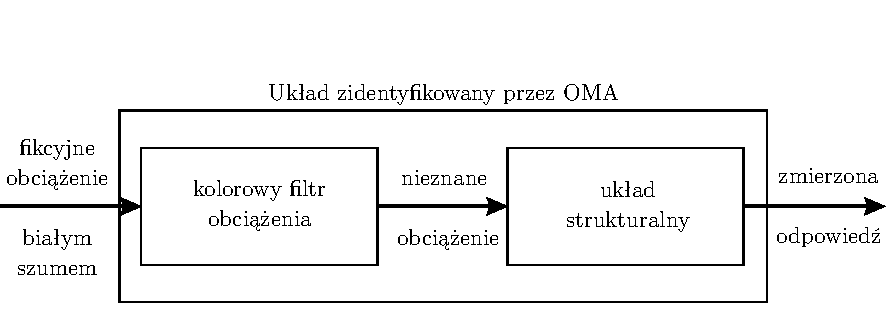
\includegraphics[]{/modal_analysis/filter_coloring.pdf}
	\captionsetup{justification=centering}
	\caption{Schemat układu identyfikowanego przez OMA przy koncepcji kolorowego filtru obciążenia}
	\label{fig: color_filter_oma}
\end{figure}

\subsection{Metody operacyjnej analizy modalnej}

Metody identyfikacji modalnej dzielą się na dwa główne rodzaje związane z dziedziną w której działa algorytm:
\begin{itemize}[noitemsep]
	\item metody w dziedzinie czasu \teng{time-domain methods (TDM)},
	\item metody w dziedzinie częstotliwości \teng{frequency-domain methods (FDM)}.
\end{itemize}
Metody EMA w dziedzinie czasu wykorzystują do estymacji parametrów modalnych funkcje odpowiedzi impulsowej \teng{inpulse response function (IRF)}. W OMA, nośnikiem informacji o odpowiedzi swobodnej układu \teng{free decays} są funkcje korelacji \teng{correlation functions}. Identyfikacja parametrów polega w tym przypadku na dopasowaniu parametrów modalnych do informacji zawartej w funkcjach korelacji. Stosowane są do tego modele parametryczne wykorzystujące techniki regresji. Główną różnicą pomiędzy dostępnymi algorytmami TD jest właśnie zastosowana metoda regresji. Zasadniczo wszystkie metody TD stosowane w EMA mogą być użyte w OMA właśnie z zastosowaniem funkcji korelacji. 


Podobną analogię jak w metodach TD można zauważyć dla metod w dziedzinie częstotliwości. W algorytmach EMA w dziedzinie częstotliwości bazą do identyfikacji są funkcje odpowiedzi częstotliwościowej \teng{frequency-response function (FRF)}. W OMA rolę tę pełnią funkcje gęstości widmowej \teng{spectral density functions}.

Przed wyborem dziedziny w której badacz chce się poruszać, warto poznać elementy charakterystyczne dla grupy algorytmów TD i FD. Podstawową wadą metod TD jest to, że wszystkie mody, które występują w sygnale są ujęte w funkcjach korelacji. W konsekwencji wszystkie mody zawsze są rozważane w trakcie rozwiązania problemu. Z kolei ich zaletą, w porównaniu do metod FD, jest większa odporność na wystąpienie błędów systematycznych w estymowanych parametrach modalnych. Niejako w kontrze do metod TD, zaletą metod FD jest to, że każdy z modów występuje w wąskim przedziale częstotliwości. Dzięki temu możliwe jest rozważanie tylko przedziałów częstotliwości, w których występują interesujące badacza mody. Z drugiej strony wadą metod FD jest wykorzystywanie do identyfikacji funkcje gęstości widmowej, które są wyznaczane za pomocą różnych metod (CYTOWANIE) obciążonych błędami systematycznymi. Błędy te nieuchronnie przenoszą się na wynikowe parametry modalne, a określenie ich wpływu jest problematyczne. \cite{Maia1997} sugerują, że metody w dziedzinie czasu są z reguły lepszym wyborem w przypadku dużego przedziału interesujących badacza częstotliwości, albo dużej liczby modów w tym zakresie. Natomiast metody w dziedzinie częstotliwości dostarczają lepszych wyników kiedy zakres częstotliwości jest niewielki, a liczba modów relatywnie mała. 

Drugie kryterium podziału algorytmów dotyczy liczby modów, które mogą być jednocześnie analizowane za pomocą danej metody. Podział jest zbliżony do tego dotyczącego teoretycznej analizy modalnej. Metoda może identyfikować albo jeden stopień swobody \teng{single degree-of-freedom} albo wiele stopni swobody \teng{multiple degree-of-freedom}.

Metody TDM i FDM możemy podzielić również na bezpośrednie \teng{direct} i pośrednie \teng{indirect}. Różnica polega na sposobie wyznaczania FRF. Metody bezpośrednie pozwalają wyznaczyć ją bezpośrednio z równania ruchu. Natomiast metody pośrednie estymują FRF na podstawie wcześniej zidentyfikowanego modelu modalnego.

Ostatnim ogólnie przyjętym kryterium podziału jest liczba punktów poddanych wymuszeniu i mierzonych w trakcie serii pomiarowej. Koresponduje to z liczbą analizowanych jednocześnie przez metodę identyfikacji funkcji FRF. Kiedy mówimy o jednoczesnej analizie tylko jednej funkcji FRF mamy do czynienia z metodą jedno-wejście-jedno-wyjście (SISO) \teng{single-input-single-output}. Kiedy mierzymy wymuszenie w jednym punkcie, a odpowiedź badamy w kilku różnych punktach na konstrukcji, otrzymując kilka funkcji FRF, metodę klasyfikuje się jako jedno-wejście-wiele-wyjść (SIMO) \teng{single-input-multi-output}. W powyższej technice obowiązuje założenie, że parametry modalne uzyskane z każdej funkcji FRF będą takie same. Innymi słowy są to parametry globalne dla całej konstrukcji. Naturalnym rozwinięciem są metody które mogą analizować wszystkie dostępne funkcje FRF jednocześnie, uzyskane w skutek wymuszenia i pomiaru wielu różnych punktów. Metody te określane są jako wiele-wejść-wiele-wyjść (MIMO) \teng{multi-input-multi-output}.

\cite{Maia1997} opisali szczegółowo wiele z metod zarówno eksperymentalnej jaki i doświadczalnej analizy modalnej. Z kolei \cite{Brincker2015} sklasyfikowali najpopularniejsze, używane współcześnie metody identyfikacji OMA. Spośród algorytmów działających w dziedzinie czasu należy wymienić:
\begin{itemize}[noitemsep]
\item Poly Reference (PR) \parencite{Norton2009,Vold1982},
\item Autoregressive Moving Average (ARMA) \parencite{Shi1987,Huang2000,Giorcelli1994},
\item Ibrahim Time Domain (ITD) \parencite{Ibrahim1983,Pappa1985a},
\item Eigensystem Realization Algorithm (ERA) \parencite{Juang1985,Pappa1985,Juang1988},
\item Stochastic Subspace Identification (SSI). \parencite{VanOverschee1996,Peeters1999a,Peeters2000}. 
\end{itemize}

Warto zaznaczyć, żę metoda ERA przy zastosowaniu postulatów NExT stanowi jeden z pośrednich wariantów metody SSI, używający funkcji korelacji jako źródła informacji przy identyfikacji.

Z kolei najpopularniejsze algorytmy w dziedzinie częstotliwości to:
\begin{itemize}[noitemsep]
\item Basic Frequency Domain (Peak-Picking) \parencite{Felber1994},
\item Frequency-Domain-Decomposition (FDD) \parencite{Brincker2000,Brincker2001a,Brincker2001b},
\item The Least Squares Complex Frequency Method (LSCF) \parencite{Verboven2005},
\item The Poly-Reference Least Squares Complex Frequency Method (p-LSCF) \parencite{Peeters2005}.
\end{itemize}



Wszystkie z powyższych algorytmów są bardzo dobrze opisane i udokumentowane w literaturze. Trudno orzec, który z nich jest obiektywnie najlepszy. Wiele zależy od doświadczenia i wiedzy autora oraz specyfiki zadania. Jak powiedział Sam Ibrahim: "Jeśli nie występują blisko położone mody i szum - wszystko zadziała" \teng{"If there are no closely spaced modes and no noise - everything works"}. Wybór metody może więc zależeć od preferencji, umiejętności programowania czy dostępnych narzędzi. W literaturze można napotkać wiele indywidualnych aplikacji algorytów (CYTOWANIE). Istnieją również komercyjne programy, które pozwala na identyfikację modalną. Do najpopularniejszych należą ARTeMIS - SVS \parencite{Extractor1999} i MACEC - dodatek do programu MATLAB \parencite{Reynders2014}.

Do identyfikacji parametrów modalnych konstrukcji, które są częścią tej pracy autor zdecydował o zastosowaniu algorytmu NExT-ERA. Wynika to z doświadczenia zespołu mostów Politechniki Gdańskiej przy stosowaniu tej metody oraz z dostępnej szerokiej literatury pokazującej skuteczne zastosowanie tej metody w przypadku badania mostów. W kolejnym rozdziale omówiono szczegóły metody oraz implementację jej algorytmu w autorskiej aplikacji napisanej w języku python.

\section{Metoda NExT-ERA}
Metoda NExT-ERA jest jedną z metod operacyjnej analizy modalnej. Składnik NExT pochodzi od słów \textbf{N}atural \textbf{Ex}citation \textbf{T}echnique. NExT jest właściwie klasą metodą OMA. Zawiera w sobie algorytmy początkowo stworzone do eksperymentalnej analizy modalnej wejście-wyjście \teng{input-output} (np. ERA, LSCE, ITD), a które następnie rozszerzone zostały do analizy problemu jedynie na podstawie sygnałów odpowiedzi konstrukcji \teng{output-only}. Taką możliwość ujawniło odkrycie faktu, że funkcje korelacji odpowiedzi konstrukcji, wywołanej losowymi wymuszeniami mogą być wyrażone jako suma zanikających sinusoid. Potwierdzono również, że funkcje korelacji zawierają informację na temat parametrów modalnych struktury. Zauważono więc, że można zastąpić tradycyjnie używane funkcje odpowiedzi impulsowej (IRF), funkcjami korelacji losowych drgań konstrukcji pod wymuszeniem środowiskowym. W ten sposób tradycyjne metody EMA zostały skutecznie zaadaptowane do OMA \parencite{Rainieri2014}. W dalszej części rozdziału zostaną przedstawione najważniejsze zagadniania dotyczące identyfikacje metodą NExT-ERA. 

\subsection{Funkcje korelacji, a odpowiedź swobodna układu}
Przyjmijmy, że $X$ oznacza zmienną losową, a $x(t)$ realizację tej zmiennej losowej w czasie. $x(t)$ w tej pracy może być utożsamiany z zaobserwowanym sygnałem. Wprowadźmy prostą definicję kowariancji. Jest to funkcja, która dostarcza informacji o zależności pomiędzy dwoma zmiennymi i dana jest wzorem:
\begin{equation}
	\mathrm{cov}[X,Y] = \mathrm{E}[XY]=\int_{-\infty}^{\infty}\int_{-\infty}^{\infty}xyp_{xy}(x,y)\,dxdy
\end{equation}
gdzie: $\mathrm{E}[\,]$ - wartość oczekiwana, $p_{xy}(x,y)$ - wspólna funkcja gęstości prawdopodobieństwa \teng{joint probability density function}. Używając metody uśredniania w czasie $[0,T]$ możemy zapisać kowariancję jako:
\begin{equation}
	\mathrm{cov}[x(t),y(t)] = \mathrm{E}[x(t)y(t)]=\frac{1}{T}\int_{0}^{T}x(t)y(t) \,dt
\end{equation}
Korelacją możemy określić zależność jak dla kowariancji, w której usunięto czynnik stały (wartość średnią) i opisać równaniem (\ref{eq: correlationDef}). W OMA zwykle sygnały na samym początku analizy są pozbawiane czynnika stałego, stąd użycie właśnie funkcji korelacji jest dla tej rodziny metod analizy modalnej kluczowe.
\begin{equation} \label{eq: correlationDef}
	\mathrm{cor}[x(t),y(t)] = \mathrm{E}[(x(t)-\mu_x)(y(t)-\mu_y)]=\frac{1}{T}\int_{0}^{T}(x(t)-\mu_x)(y_{}(t)-\mu_y) \,dt
\end{equation}

W OMA funkcja korelacji wykorzystywana jest jako autokorelacja \teng{autocorrelation} i cross-korelacja \teng{cross-correlation}. Dla pojedynczego sygnału $x(t)$ można rozważyć jak wygląda korelacja pomiędzy punktem $x(t)$, a punktem $x(t+\tau)$, czyli odległym w czasie o $\tau$. Przedstawienie graficzne problemu pokazano na rysunku \ref{fig: autocorrelationExample}. Intuicyjnie widać, że wartość korelacji dla punktów bliskich sobie będzie duża, a dla punktów bardzo od siebie odległych będzie maleć. Autokorelacją nazwiemy funkcję daną równaniem (\ref{eq: autocorrelationDef}), gdzie funkcję $y$ w równaniu (\ref{eq: correlationDef}) zastąpiono $x(t+\tau)$. 
\begin{figure}[h] 
	\centering
	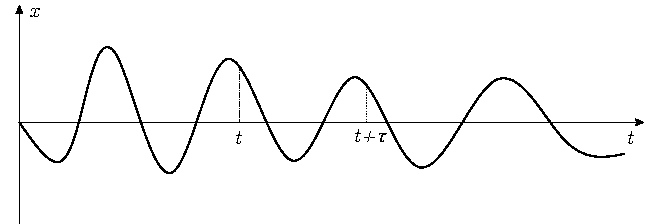
\includegraphics[]{/korelacja/korelacja.pdf}
	\captionsetup{justification=centering}
	\caption{Autokorelacja, jako korelacja wartości funkcji $x(t)$ w czasie $t$ i $t+\tau$}
	\label{fig: autocorrelationExample}
\end{figure}
\begin{equation} \label{eq: autocorrelationDef}
	R_x(\tau)=\mathrm{E}[x(t)x(t+\tau)]
\end{equation}
Funkcję cross-korelacji opiszemy analogicznie jak autokorelacji, z tą różnicą, że pod uwagę weźmiemy dwa losowe sygnały $x(t)$ i $y(t)$.
\begin{equation} \label{eq: crosscorrelationDef}
	\begin{aligned}
	R_{xy}(\tau)=\mathrm{E}[x(t)y(t+\tau)]\\	
	R_{yx}(\tau)=\mathrm{E}[y(t)x(t+\tau)]
	\end{aligned}
\end{equation}

Nie znając funkcji gęstości prawdopodobieństwa, funkcje autokorelacji  i cross-korelacji można wyznaczyć za pomocą uśredniania w czasie co opisano równaniami odpowiednio (\ref{eq: timeAveAutocorrelation}) i (\ref{eq: timeAveCrosscorrelation}). W dalszej części pracy podane zostaną inne przykłady metod wyznaczania funkcji korelacji.
\begin{equation} \label{eq: timeAveAutocorrelation}
	R_x = \frac{1}{T}\int_{0}^{T}x(t)x(t+\tau) \,dt
\end{equation}

\begin{equation} \label{eq: timeAveCrosscorrelation}
	\begin{aligned}
	R_{xy} = \frac{1}{T}\int_{0}^{T}x(t)y(t+\tau) \,dt \\
	R_{yx} = \frac{1}{T}\int_{0}^{T}y(t)x(t+\tau) \,dt 
\end{aligned}
\end{equation}
Jedną z istotnych właściwości funkcji korelacji jest możliwość wyznaczenia jej przez splot między sygnałem $x(-t)$ i $y(t)$, co zapisano równaniem (\ref{eq: splotCorrelation}). Główną zaletą tego rozwiązania jest prostota obliczeń, ponieważ splot dwóch funkcji jest łatwy do wyznaczenia w dziedzinie częstotliwości \parencite{Brincker2015}.
\begin{equation} \label{eq: splotCorrelation}
	R_{xy}(\tau)=x(-t)*y(t)
\end{equation}
W praktyce wykonywanych jest wiele pomiarów. Załóżmy, że dla zestawu $N$ pomiarów, zmierzone odpowiedzi mogą być zestawione w wektor:
\begin{equation}
\vect{y}(t) = \{y_1(t),y_2(t),y_3(t), \hdots ,y_N(t)\}^T
\end{equation}
Wyniki autokorelacji i cross-korelacji pomiędzy wszystkimi zmierzonymi sygnałami można zagregować i zapisać macierzowo (\ref{eq: matCorelationDef}). Na przekątnej macierzy znajdują się funkcje autokorelacji, a poza przekątną cross-korelacji.
\begin{equation} \label{eq: matCorelationDef}
	\matr{R}^T(\tau)=\mathrm{E}[\vect{y}(t)\vect{y}^T(t+\tau)]
\end{equation}
Macierzą korelacji \teng{correlation matrix} nazywa się macierz (\ref{eq: matCorelationDef}) dla $\tau=0$ co można zapisać wzorem (\ref{eq: correlationMatrixDef}).
\begin{equation} \label{eq: correlationMatrixDef}
	\matr{C}=\mathrm{E}[\vect{y}(t)\vect{y}^T(t)]=\matr{R}(0)
\end{equation}

Funkcje korelacji posiadają dwie wspomniane wcześniej właściwości kluczowe dla OMA. Po pierwsze teoretycznie pozwalają wyodrębnić wszystkie informacje na temat parametrów modalnych konstrukcji z sygnału losowego. Po drugie mogą być utożsamiane z drganiami swobodnymi, gasnącymi układu \parencite{James1995}. Oba założenia zostały wyjaśnione i udowodnione poniżej.

Założenie o reprezentacji wszystkich parametrów modalnych przez funkcje korelacji opiera się na wykorzystaniu właściwości funkcji korelacji, rozkładu normalnego oraz Centralnego Twierdzenia Granicznego \teng{central limit theorem}. Centralne Twierdzenie Graniczne mówi, że dla niezależnych zmiennych losowych $X_i$ o jednakowym rozkładzie, fluktuujących wokół wartości oczekiwanej $\mu$ i o skończonej wariancji $\sigma^2$ to wyrażenie (\ref{eq:centralLimitTheorem})
\begin{equation} \label{eq:centralLimitTheorem}
	\frac{\frac{1}{n}\sum_{i=1}^{M} X_i - \mu}{\frac{\sigma}{M}}
\end{equation}
zbiega według rozkładu do rozkładu Gaussa przy nieskończonej liczbie M.
\cite{Brincker2015} przedstawili uzasadnienie użycia tego twierdzenia w przypadku OMA w następujący sposób. Rozważmy zestaw zmiennych losowych $\{x_1,x_2,...,x_M\}$, które są niezależne i posiadają identyczny rozkład, ze średnią wartością $\mu$ i wariancją $\sigma^2$. Liniowa kombinacja tych zmiennych losowych jest dana wzorem:
\begin{equation} \label{eq:CLTsum}
	y = \sum_{i=1}^{M} a_i x_i
\end{equation}
 Centralne twierdzenie graniczne mówi o tym, że dla dużej liczby zmiennych losowych $M$ rozkład $y$ jest w przybliżeniu normalny, z wartością średnią $\mu_y=\mu\sum a_i$, wariancją $\sigma_y^2=\sigma^2\sum \sigma^2$ i przy $M \xrightarrow{} \infty$ zbiega do rozkładu normalnego. Odwołując się do dynamiki budowli możemy zapisać, że odpowiedź układu $y(t)$ jest splotem siły wymuszającej $x(\tau)$ i funkcji odpowiedzi impulsowej $h(t)$ co pokazano równaniem:
 \begin{equation} \label{eq:convolutionResponse}
 	y(t)=\int_{-\infty}^{\infty}h(t-\tau)x(\tau) \,d\tau
 \end{equation}
 
  Dla sygnału dyskretnego z krokiem czasowym $\Delta t$ i ograniczając się jedynie do $N_m$ istotnych z punktu widzenia pamięci systemu próbek, zależność może być przedstawiona następująco:
 \begin{equation}
 	y(n) = \sum_{k=n-N_m}^{n} h(n-k)x(k)\Delta t
 \end{equation}
Można zauważyć, że dla wymuszenia szumem białym odpowiedź dynamiczna $y(n)$ jest sumą, którą można przedstawić wzorem (\ref{eq:CLTsum}), gdzie poszczególne składniki obciążenia $x(k)$ nie muszą mieć rozkładu normalnego, ale ostateczna odpowiedź będzie mieć rozkład Gaussa. Wynika to wprost z Centralnego Twierdzenia Granicznego. Warto nadmienić, że założenie o wymuszeniu białym szumem zapewnia nam niezależność składników obciążenia $x(k)$. 

Bazując na powyższym, w OMA zwykle zakładamy, że mierzone sygnały posiadają wartość średnią równą zero oraz są Gaussowskie \teng{Gaussian signals} lub bliskie Gaussowskim \parencite{Brincker2015}. Przypomnijmy, że jednowymiarowa funkcja gęstości prawdopodobieństwa rozkładu normalnego dana jest wzorem:
\begin{equation}
	p(x) = \frac{1}{\sqrt{2\pi\sigma^2}}e^{-\frac{(x-\mu)^2}{2\sigma^2}}
\end{equation}
, a przyjmując dodatkowo wartość średnią równą
 zero wzór można wyrazić następująco:
\begin{equation} \label{eq:normalDensZeroMean}
	p(x) = \frac{1}{\sqrt{2\pi\sigma^2}}e^{-\frac{x^2}{2\sigma^2}}
\end{equation}
Dla wektora losowego, zawierającego zmienne losowe o zerowej wartości średniej $\vect{x}^T=\{x_1,x_2,x_3,\hdots,x_M\}$, funkcja gęstości prawdopodobieństwa może być zapisana jako:
\begin{equation}\label{eq: normalDistributionCorr}
	p(x) = \frac{1}{(2\pi)^\frac{M}{2} \matr{|C|}}e^{\vect{x}^T\matr{C}^{-1}\vect{x}/2}
\end{equation}
gdzie $|\matr{C}|$ jest wyznacznikiem macierzy korelacji (\ref{eq: correlationMatrixDef}). Podstawowym wnioskiem wynikającym z tej zależności jest to, że jednowymiarowy rozkład Gaussa może być opisany za pomocą średniej wartości, odchylenia standardowego i w przypadku wielowymiarowych danych o zerowej wartości średniej, jedynie przez przez macierz korelacji (\ref{eq: normalDistributionCorr}).

Aby wytłumaczyć dlaczego funkcje korelacji w OMA mogą być odpowiednikiem funkcji odpowiedzi impulsowej (IRF), a funkcje gęstości widmowej odpowiednikami funkcji odpowiedzi częstotliwościowej (FRF) przytoczmy wymagane definicje i zależności z dynamiki budowli. Szczegółowe wyprowadzenia i objaśnienia znajdują się między innymi w pracach \parencite{Brincker2015,Rainieri2014,Chopra2012a,Ewins2000}. Funkcja odpowiedzi impulsowej układu, zwykle oznaczone jako $h(t)$ jest odpowiedzią układu poddanego wymuszeniu przez impulsową siłę, o bardzo krótkim czasie działania, w chwili czasowej $t=0$. Matematycznie impulsową siłę opisuje funkcja nazywaną deltą Diraca $\delta(t)$. Dla systemów liniowych i czasowo niezależnych, jeżeli przesunięta w czasie zostanie chwila przyłożenia impulsu o $\tau$, to otrzymamy odpowiedź $y(t)$, która będzie również przesunięta w czasie o $\tau$. Z definicji wiemy, że impuls jest iloczynem intensywności obciążenia i czasu jego działania. Rozważmy ciągłe obciążenie oznaczone jako $x(t)$, które jest superpozycją potoku impulsów o zmiennej amplitudzie, ale o równie krótkich czasach trwania. W takim przypadku impuls siły od czasu $\tau$ do $\tau+d\tau$ obliczamy jako $x(\tau)d\tau$, a odpowiedź układu jako $h(t-\tau)x(\tau)d\tau$. Układ jest liniowy a więc obowiązuje zasada superpozycji. Wynika z tego, że suma wpływu całego obciążenia może być wyznaczona jako suma wszystkich składowych odpowiedzio i opisana całką Duhamel'a jako (\ref{eq: duhamelIntegralIRF}) oraz w postaci splotu (\ref{eq: convolutionIntegralIRF}) miedzy funkcją IRF $h(t)$ i wymuszeniem $x(t)$.
\begin{equation} \label{eq: duhamelIntegralIRF}
	y(t)=\int_{-\infty}^{\infty} h(t-\tau)x(\tau)d\tau
\end{equation}
\begin{equation} \label{eq: convolutionIntegralIRF}
	y(t)=h(t)*x(t)
\end{equation}
Funkcję IRF można wyznaczyć wykonując przekształcenie Laplace'a równania ruchu przedstwaionego równaniem (\ref{eq: mot_und}). Dla przejrzystości przytoczono je poniżej (\ref{eq: motionIRF}), dla układu z jednym stopniem swobody, wymuszenia deltą Diraca i podstawiając w miejsce odpowiedzi układu funkcję IRF:
\begin{equation} \label{eq: motionIRF}
	m\ddot{h}(t)+c\dot{h}(t)+kh(t)=\delta(t)
\end{equation}
Wykonując transformatę Laplace'a obu stron otrzymamy:
\begin{equation} \label{eq: laplaceTransofrmMOVEQ}
	(ms^2+cs+k)H(s)=1
\end{equation}
Wykorzystując właściwości transformaty i przekształcając odpowiednio równanie (\ref{eq: laplaceTransofrmMOVEQ}) otrzymamy formułę (\ref{eq: laplaceTransofrmMOVEQ2}). Na jej podstawie można wprost wyznaczyć funkcje IRF podaną równaniem (\ref{eq: IRFfunction}).
\begin{equation} \label{eq: laplaceTransofrmMOVEQ2}
	H(s) = \frac{1}{m(s-\lambda)(s-\lambda^*)}
\end{equation}
\begin{equation} \label{eq: IRFfunction}
	h(t)=\frac{1}{m}\frac{e^{\lambda t}-e^{\lambda^*t}}{\lambda-\lambda^*}
\end{equation}



Z kolei funkcja FRF w sensie fizycznym reprezentuje amplitudę i przesunięcie fazowe drgań ustalonych systemu SDOF, poddanego wymuszeniu harmonicznemu o jednostkowej amplitudzie i częstotliwości $\omega_d$. Matematycznie FRF $H(\omega)$ można opisać również jako transformatę Laplace'a z IRF obliczoną dla urojonej współrzędnej $s=i\omega$ (\ref{eq: laplaceTransofrmMOVEQ2}) i zapisać następująco:
\begin{equation} \label{eq: FRFfunction}
	H(\omega)=\frac{1}{m(i\omega-\lambda)(i\omega-\lambda^*)}
\end{equation}
Podobnie jak IRF, FRF łączy wymuszenie z odpowiedzią układu. Jeśli równanie ruchu (\ref{eq: mot_und}) stronami przekształcimy transformatą Fouriera to otrzymamy:
\begin{equation} \label{eq: FRF_moteq}
	(m(i\omega)^2+ci\omega + k)Y(\omega)=X(\omega)
\end{equation}
Szczegółowe rozwiązanie za pomocą reprezentacji biegunów układu można znaleźć w literaturze \parencite{Brincker2015}. Ostatecznie otrzymujemy:
\begin{equation} 
	m(i\omega-\lambda)(i\omega-\lambda^*)Y(\omega)=X(\omega)
\end{equation}
Po przekształceniu wyraźnie widać relację pomiędzy odpowiedzią, a wymuszeniem układu za pośrednictwem FRF:
\begin{equation} \label{eq: FRF_final}
	Y(\omega)=\frac{1}{m(i\omega-\lambda)(i\omega-\lambda^*)}X(\omega)=H(\omega)X(\omega)
\end{equation}
gdzie $X(\omega)$ i $Y(\omega)$ są odpowiednio transformatami Fouriera wymuszenia $x(t)$ i odpowiedzi $y(t)$ układu. Porównując równania (\ref{eq: FRF_moteq})(\ref{eq: FRF_final}) łatwo można zauważyć że FRF zawiera w sobie informację na temat bezwładności, tłumienia i sztywności układu.




Zarówno IRF jak i FRF można uogólnić do układów MDOF o $N$ stopniach swobody. Zapis zależności wymuszenie-odpowiedź dla układu MIMO (wiele-wejść-wiele-wyjść) przedstawiono dla dziedziny czasu (\ref{eq: mimoIRFyx}) i częstotliwości (\ref{eq: mimoFRFyx}).

\begin{equation} \label{eq: mimoIRFyx}
	\vect{y}(t)=\matr{H}(t)*\vect{x}(t)
\end{equation}
\begin{equation} \label{eq: mimoFRFyx}
	\vect{\tilde{y}}(\omega)=\matr{\tilde{H}}(i\omega)\vect{\tilde{x}}(\omega)
\end{equation}
gdzie $\matr{H}(t)$ jest macierzą zawierającą funkcje IRF, $\vect{x}(t)$ jest wektorem sił wymuszających, $\vect{\tilde{y}}(\omega)$ i $\vect{\tilde{x}}(\omega)$ są transformatami Fouriera odpowiednio $\vect{x}(t)$ i $\vect{y}(t)$, a $\matr{\tilde{H}}(i\omega)$ jest macierzą FRF. Wyrażenia na odpowiednio IRF $\matr{H}(t)$ i FRF $\matr{\tilde{H}}(i\omega)$ podano poniżej.
\begin{equation}
	\matr{H}(t)=\sum_{n=1}^{N}(\vect{A}_n e^{\lambda_n t} + \vect{A}_n^* e^{\lambda_n t})
\end{equation}
\begin{equation}
	\matr{\tilde{H}}(i\omega)=\sum_{n=1}^{N}(\frac{\vect{A}_n}{i\omega-\lambda_n} + \frac{\vect{A}_n^*}{i\omega-\lambda_n^*})
\end{equation}
gdzie $\vect{A}_n=Q_n \vect{\psi}_n\vect{\psi}_n^T$, $\vect{\psi}_n$ to n-ta postać drgań własnych, $Q_n$ to współczynnik skalujący mody, a $\lambda_n=\sigma_n+i\omega_{d,n}$ jest n-tym biegunem układu zawierającym informacje na temat częstotliwości drgań własnych tłumionych $f_{d,n}=\omega_{d,n}/(2\pi)$ i liczby tłumienia $\xi_r=-\sigma_n/\sqrt{\sigma_n^2+\omega_{d,n}^2}$ n-tego moda.






Gęstość widmowa jest kolejnym kluczowym pojęciem potrzebnym do pełnego zrozumieniu znaczenia funkcji korelacji dla OMA. Gęstość widmowa \teng{auto spectral density} dla przebiegu czasowego $x(t)$ jest zdefiniowana jako transformata Fouriera z funkcji korelacji $R_x(\tau)$ \ref{eq: spectralDensity}. Istnieje również zależność odwrotna, w której odwrotną transformata Fouriera z gęstości widmowej pozwala otrzymać funkcję korelacji \ref{eq: correlationInversSpectralDensity}. Początkowy wyraz funkcji korelacji $R_x(0)$ jest reprezentacją twierdzenia Parsevela i pozwala stwierdzić, że gęstość widmowa pokazuje rozkład energii w funkcji częstotliwości. Stąd gęstość widmową nazywa się również zamiennie gęstością widmową mocy \teng{power spectral density} (PSD) \parencite{Brincker2015}.
\begin{equation} \label{eq: spectralDensity}
	G_x(\omega) = \frac{1}{2\pi}\int_{-\infty}^{\infty}R_x(\tau)e^{-i\omega\tau}\,d\tau
\end{equation}
\begin{equation} \label{eq: correlationInversSpectralDensity}
	R_x(\omega) = \int_{-\infty}^{\infty}G_x(\omega)e^{i\omega\tau}\,d\omega
\end{equation}
Podobnie zdefiniować można gęstość widmową pomiędzy dwoma sygnałami $x(t)$ i $y(t)$ \teng{cross spectral density}, jako przekształcenie Fouriera funkcji cross-korelacji $R_{xy}(t)$. 

\begin{equation} \label{eq: crossspectralDensity}
	G_{xy}(\omega) = \frac{1}{2\pi}\int_{-\infty}^{\infty}R_{xy}(\tau)e^{-i\omega\tau}\,d\tau
\end{equation}
\begin{equation} \label{eq: crosscorrelationInversSpectralDensity}
	R_{xy}(\omega) = \int_{-\infty}^{\infty}G_{xy}(\omega)e^{i\omega\tau}\,d\omega
\end{equation}
Wykorzystanie właściwości splotu funkcji korelacji (\ref{eq: splotCorrelation}) i  splotu\footnote{Transformata Fouriera splotu dwóch funkcji w dziedzinie czasu $h(t)$ i $g(t)$ jest równa iloczynowi transformat Fouriera każdej z funkcji osobno. Innymi słowy transformacie Fouriera wyrażenia $h(t)*g(t)$ odpowiada iloczyn $H_k G_k$, gdzie: $H_k$ - transformata Fouriera funkcji $h(t)$, $G_k$ - transformata Fouriera funkcji $g(t)$.} oraz symetrii Hermitowskiej\footnote{Jeżeli $H(\omega)$ jest transformatą Fouriera rzeczywistej funkcji $h(t)$, to prawdziwe jest równanie $H(\omega)=H^*(-\omega)$. Równanie to jest nazywane symetrią Hermitowską \parencite{Boashash2015}.} transformaty Fouriera pozwala uzyskać następującą właściwość gęstości widmowej (\ref{eq: specDensSplot}). Należy nadmienić, że zależność ta będzie spełniona przy założeniu okresowego (lub bardzo długiego) sygnału \parencite{Brincker2015}.
\begin{equation} \label{eq: specDensSplot}
	G_{xy}(\omega) = X^*(\omega)Y(\omega)
\end{equation}


Rozważamy ponownie układ SISO o odpowiedzi $y(t)$ przy wzbudzeniu $x(t)$: $y(t)=x(t)*h(t)$ (\ref{eq: convolutionIntegralIRF}). Wykorzystując równanie (\ref{eq: specDensSplot}) zapiszemy równanie na gęstość widmową odpowiedzi:
\begin{equation} \label{g}
	G_{y}(\omega) = Y^*(\omega)Y(\omega)
\end{equation}
Wykorzystując transformatę FOuriera oraz przemienność i łączność splotu zapisać można następujące równanie pokazujące zależność pomiędzy gęstością widmową odpowiedzi i wymuszenia układu.
\begin{equation}
	G_{y}(\omega) = G_x(\omega)|H^*(i\omega)|^2
\end{equation}
Równanie to jest nazywane twierdzeniem podstawowym \teng{fundamental theorem} metody OMA. Dla układu MIMO twierdzenie to przyjmuje następującą formę:
\begin{equation}
	\begin{split}
	\matr{G}_{y}(\omega) &=\matr{\tilde{H}}^*(i\omega)\matr{G}_x(\omega)\matr{\tilde{H}}^T(i\omega)\\
	&=\matr{\tilde{H}}^*(i\omega)\matr{G}_x(\omega)\matr{\tilde{H}}^T(i\omega)
	\end{split}
\end{equation}

Za










\subsection{Eigenystem Realization Algorithm}

\subsection{Elementy przetwarzania sygnałów}


	\chapter{Metody analizy modalnej}

	Podział metod (diagram)
	\section{Metoda ERA}
	\section{Metoda NEXT-ERA}
	\section{Implementacja programu}
MAC - \parencite{allemang_modal_2003} formuła musi być dla zespolonych a nie tylko transpozycja!
\section{Testy numeryczne metody NEXT-ERA}
\section{Testy eksperymentalne metody NEXT-ERA}
